\let\negmedspace\undefined
\let\negthickspace\undefined
\documentclass[journal]{IEEEtran}
\usepackage[a5paper, margin=10mm, onecolumn]{geometry}
%\usepackage{lmodern} % Ensure lmodern is loaded for pdflatex
\usepackage{tfrupee} % Include tfrupee package

\setlength{\headheight}{1cm} % Set the height of the header box
\setlength{\headsep}{0mm}     % Set the distance between the header box and the top of the text

\usepackage{gvv-book}
\usepackage{gvv}
\usepackage{cite}
\usepackage{amsmath,amssymb,amsfonts,amsthm}
\usepackage{algorithmic}
\usepackage{graphicx}
\usepackage{textcomp}
\usepackage{xcolor}
\usepackage{txfonts}
\usepackage{listings}
\usepackage{enumitem}
\usepackage{mathtools}
\usepackage{gensymb}
\usepackage{comment}
\usepackage[breaklinks=true]{hyperref}
\usepackage{tkz-euclide} 
\usepackage{listings}
% \usepackage{gvv}                                        
\def\inputGnumericTable{}                                 
\usepackage[latin1]{inputenc}                                
\usepackage{color}                                            
\usepackage{array}                                            
\usepackage{longtable}                                       
\usepackage{calc}                                             
\usepackage{multirow}                                         
\usepackage{hhline}                                           
\usepackage{ifthen}                                           
\usepackage{lscape}
\begin{document}

\bibliographystyle{IEEEtran}

\title{2.4.18}
\author{EE25BTECH11023 - Venkata Sai}
% \maketitle
% \newpage
% \bigskip
{\let\newpage\relax\maketitle}

\renewcommand{\thefigure}{\theenumi}
\renewcommand{\thetable}{\theenumi}
\setlength{\intextsep}{10pt} % Space between text and floats


\numberwithin{align}{enumi}
\numberwithin{figure}{enumi}
\renewcommand{\thetable}{\theenumi}


\textbf{Question}:\newline
Find the values of $\vec{p}$ so that the lines $\frac{1-x}{3} = \frac{7y-14}{2p} = \frac{z-3}{2}$ and $\frac{7-7x}{3p} = \frac{y-5}{1} = \frac{6-z}{5}$ are at right angles. 
\\
\textbf{Solution: }
\begin{table}[H]    
  \centering
  

  \caption{Variables Used}
\end{table} 
Line 1:
\begin{align}
\frac{1-x}{3} = \frac{7y-14}{2p} = \frac{z-3}{2} \implies \frac{x-1}{-3} = \frac{y-2}{\frac{2p}{7}} = \frac{z-3}{2}
\end{align}
Line 2:
\begin{align}
\frac{7-7x}{3p} = \frac{y-5}{1} = \frac{6-z}{5} \implies \frac{x-1}{-\frac{3p}{7}} = \frac{y-5}{1} = \frac{z-6}{-5}
\end{align}
Direction vector for line 1:
\begin{align}
m_1 = \myvec{-3 \\ \frac{2p}{7} \\ 2}
\end{align}
Direction vector for line 2:
\begin{align}
m_2 = \myvec{-\frac{3p}{7} \\ 1 \\ -5}
\end{align}
Since the lines are at right angles
\begin{align}
\myvec{m_1}^\top\myvec{m_2} = 0 \\
\myvec{-3 \ \frac{2p}{7} \ 2}\myvec{-\frac{3p}{7} \\ 1 \\ -5}=0
\end{align}
\begin{align}
(-3)(-\frac{3p}{7}) + (\frac{2p}{7})(1) + (2)(-5) = 0
\end{align}
\begin{align}
p = \frac{70}{11}
\end{align}
Hence the value of $\vec{p}$ is $\frac{70}{11}$
\begin{figure}[h!]
   \centering
   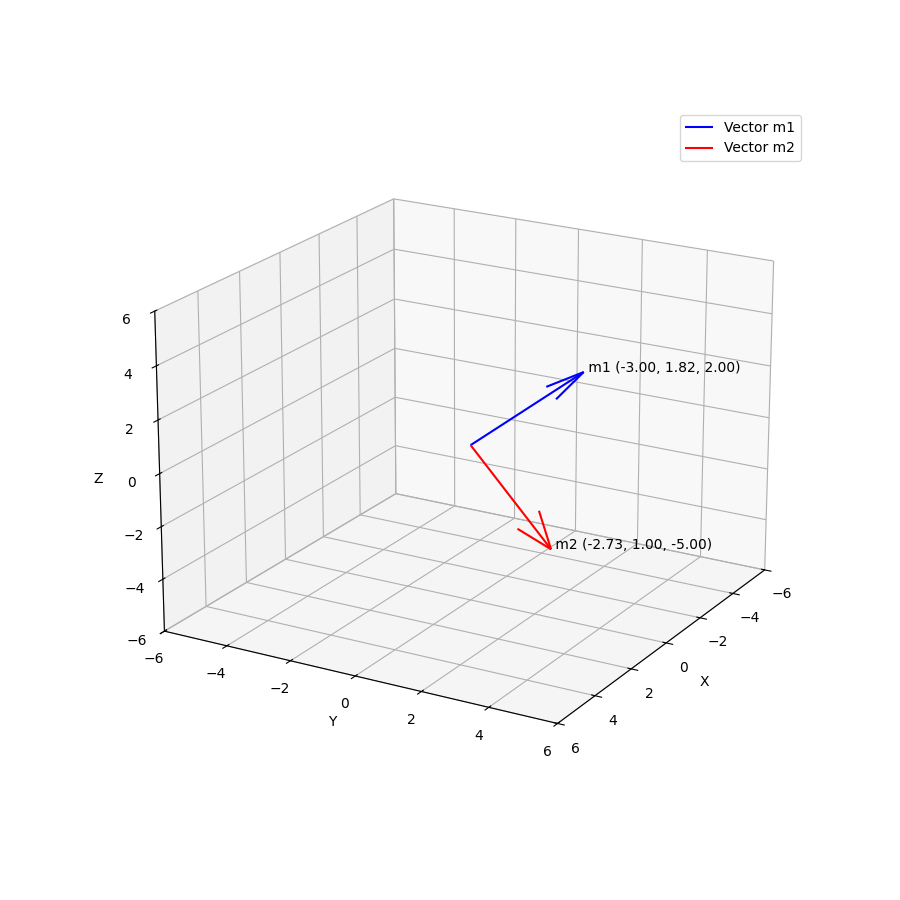
\includegraphics[width=0.7\columnwidth]{figs/fig1.png}
   \caption{Stem Plot of y\brak{n}}
   \label{stemplot}
\end{figure}
\end{document}  